\begin{figure*}[htb]
  \centering
  \begin{subfigure}[b]{0.475\textwidth}
    \centering
    \includegraphics[width=\textwidth]{figures/des/7-2-2.png}
    \caption{ID 7-2-2}
  \end{subfigure}%
  \hfill
  \begin{subfigure}[b]{0.475\textwidth}
    \centering
    \includegraphics[width=\textwidth]{figures/des/1-5.png}
    \caption{ID 1-5}
  \end{subfigure}
  \vskip\baselineskip

  \begin{subfigure}[b]{0.475\textwidth}
    \centering
    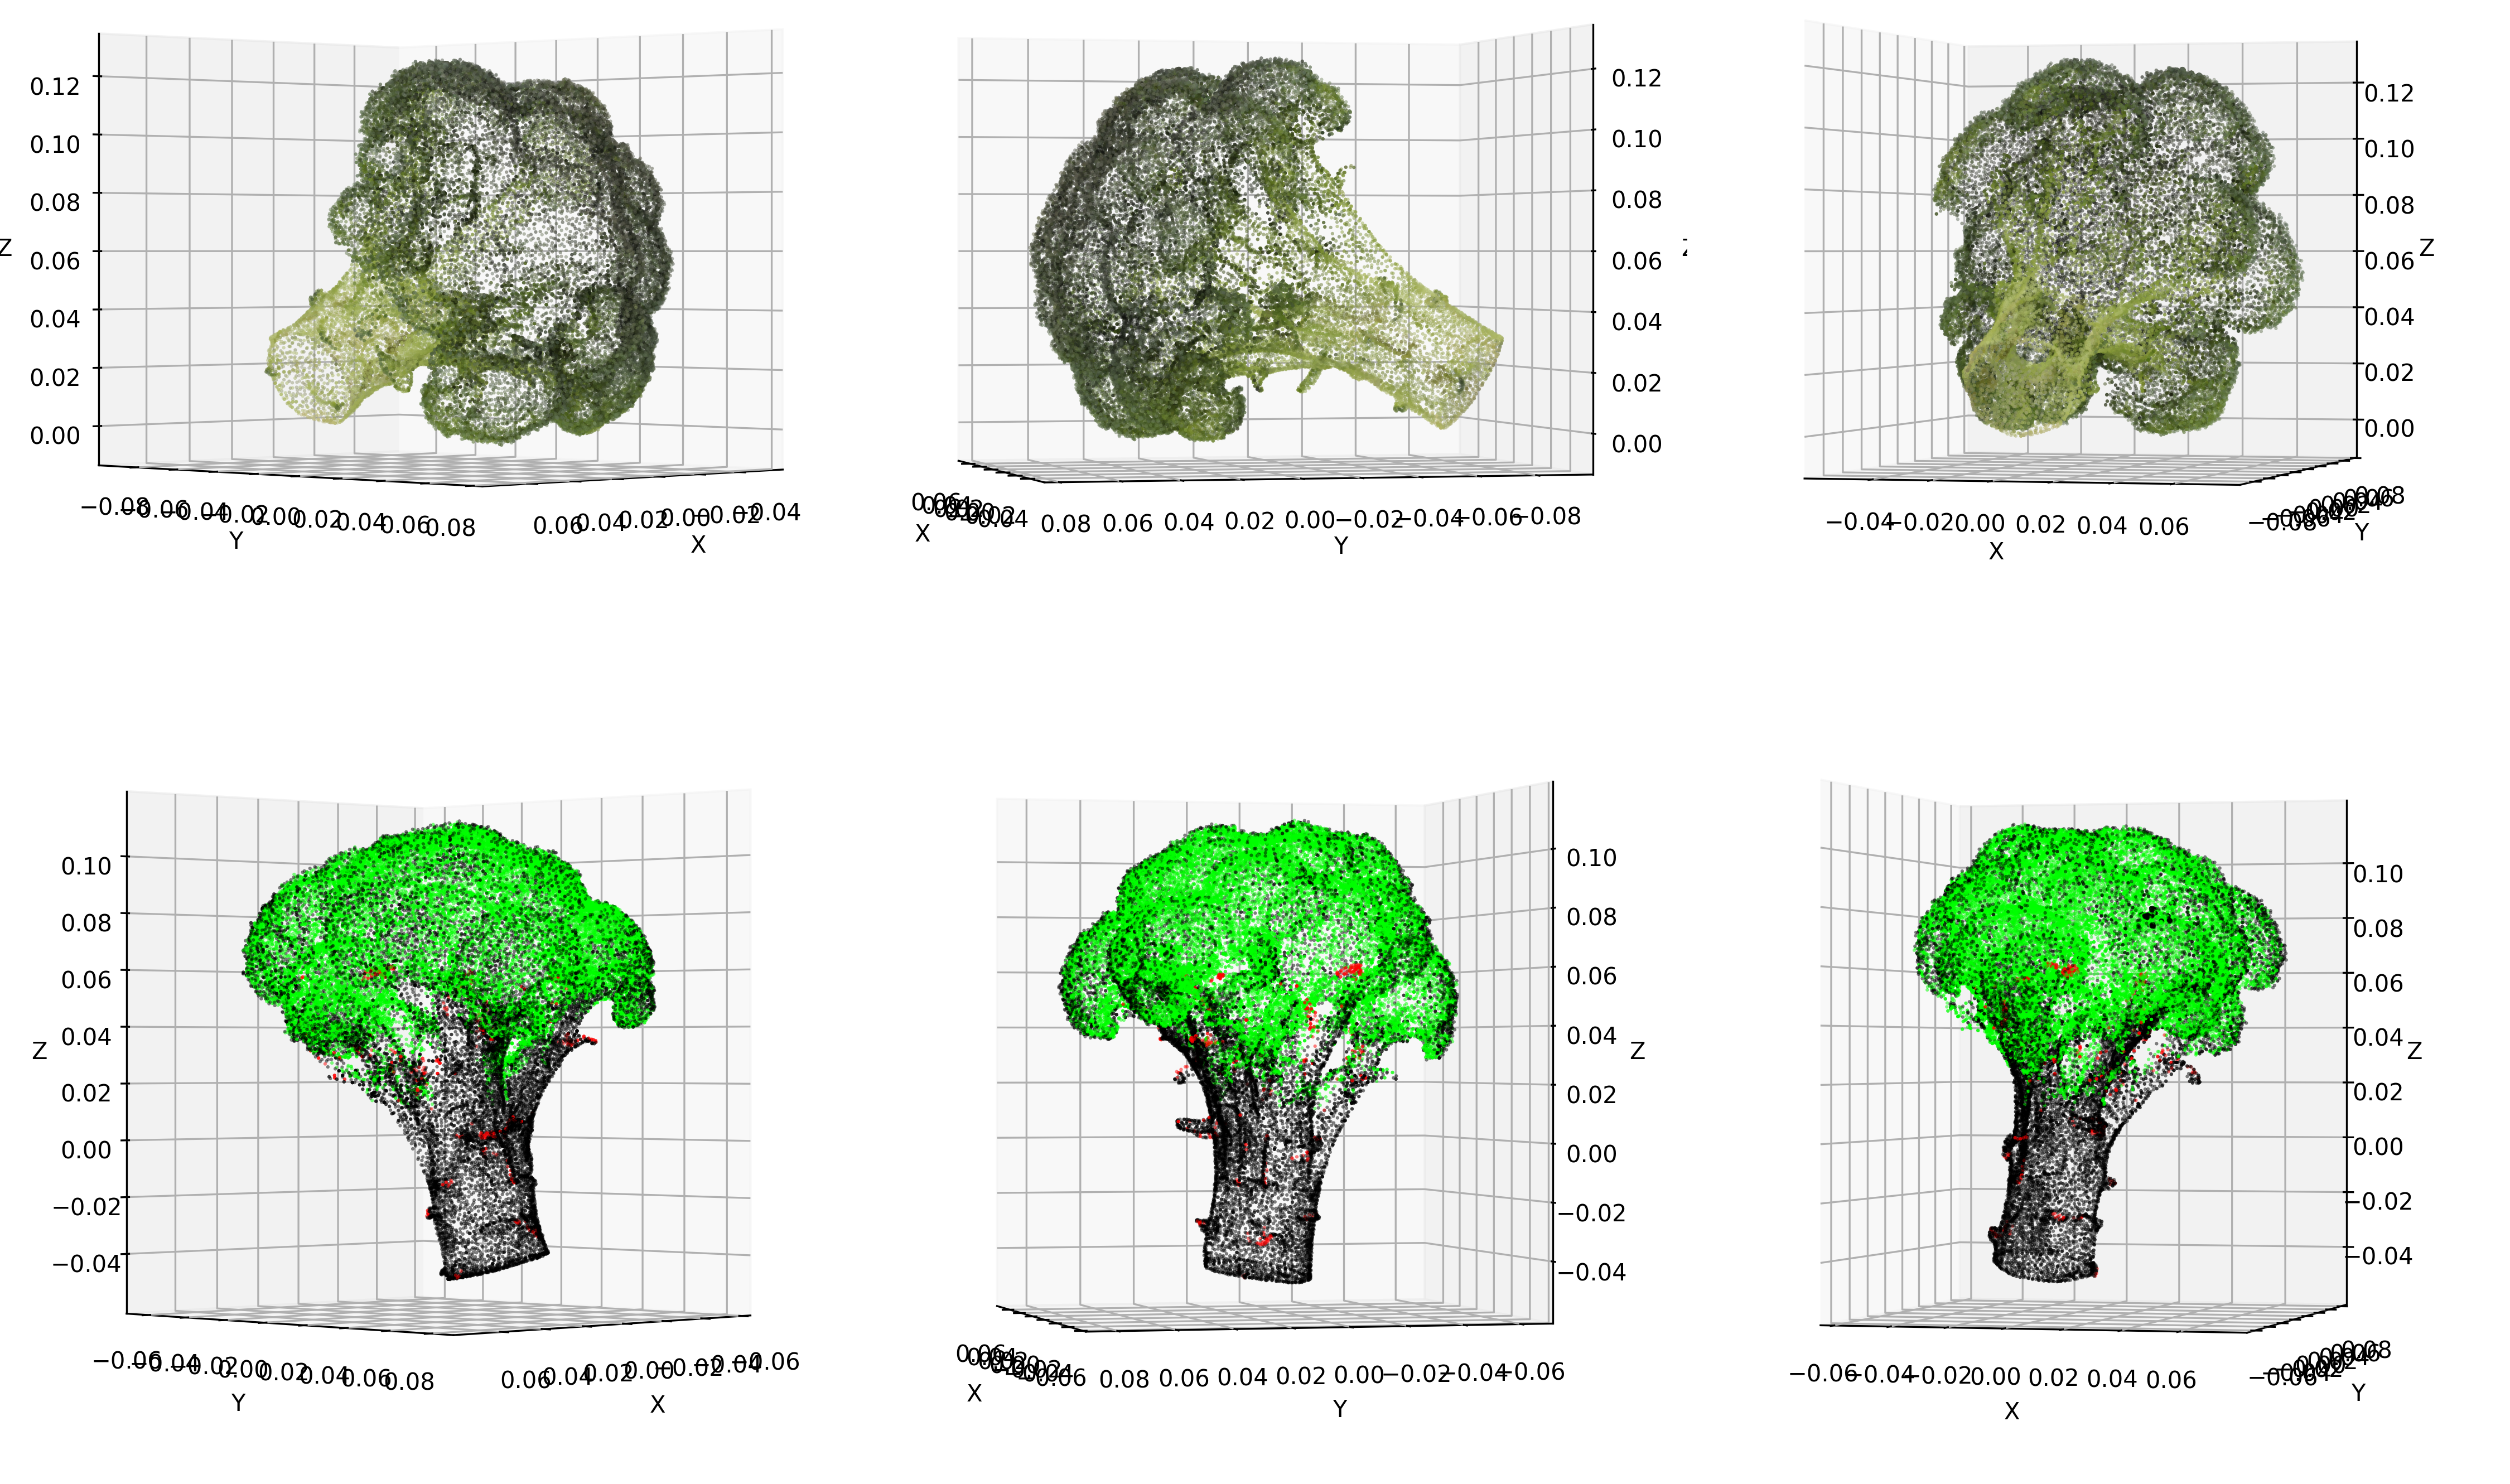
\includegraphics[width=\textwidth]{figures/des/2-23.png}
    \caption{ID 2-23}
  \end{subfigure}%
  \hfill
  \begin{subfigure}[b]{0.475\textwidth}
    \centering
    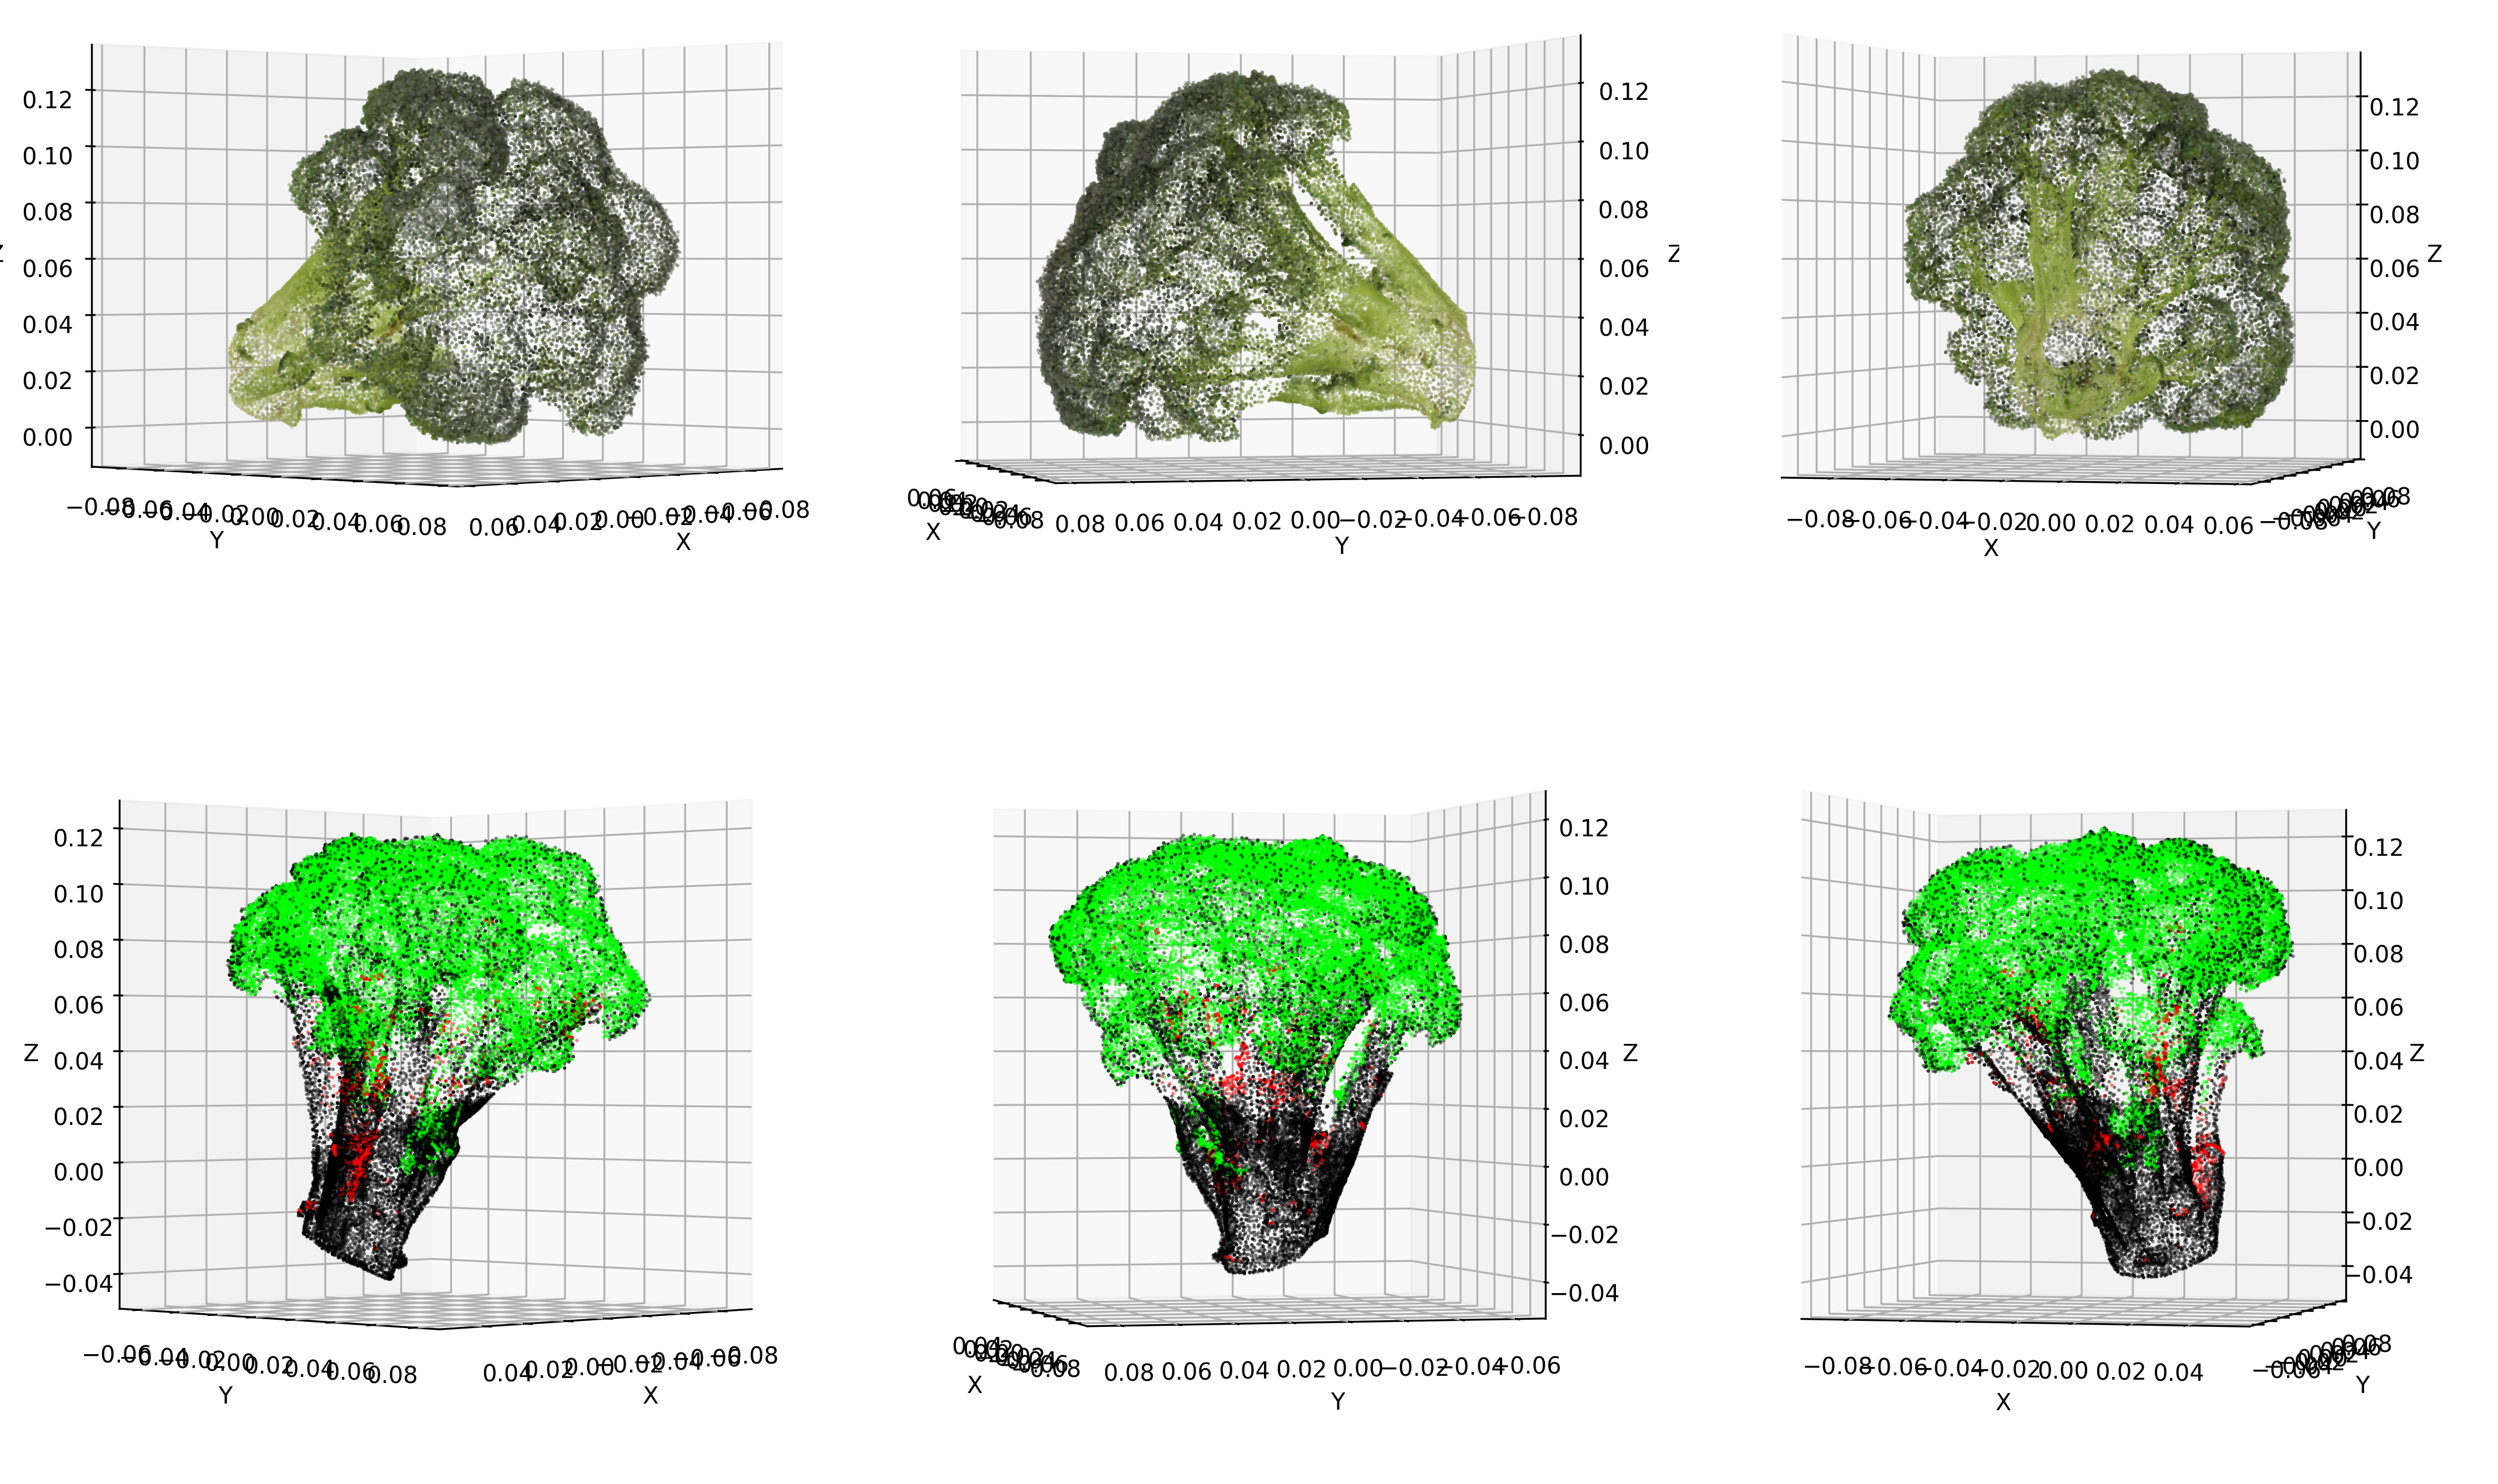
\includegraphics[width=\textwidth]{figures/des/1-33.png}
    \caption{ID 1-33}
  \end{subfigure}%
  \caption[Examples of plant 3D model analysis at different growing stages]{
    Examples of plant 3D model analysis at different growing stages. The upper parts are the original coordinates of the obtained 3D models, while the lower parts are the segmented and direction-corrected results, the red parts are removed noises. Three columns show the corresponding azimuth angle views at $45^\circ$, $165^\circ$, and $285^\circ$ for the same 3D model.
  }
  \label{fig:des6}
\end{figure*}